\documentclass[tikz]{standalone}
\usetikzlibrary{arrows.meta,math}
\usepackage{xcolor}
\begin{document}
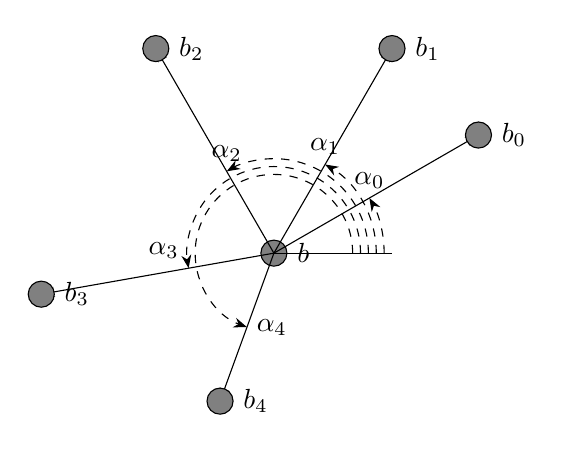
\begin{tikzpicture}[>=Stealth]
	\node[circle,fill=black!50,draw,label=right:$b$]{};
	\draw (0,0)--(right:1.5cm);
	\foreach \n/\d/\l/\a/\r/\p in { 
			0/1.4cm/b_0/30/3cm/above, 
			1/1.3cm/b_1/60/3cm/above, 
			2/1.2cm/b_2/120/3cm/above,
			3/1.1cm/b_3/190/3cm/above left,
			4/1.0cm/b_4/250/2cm/right}
		{
		\draw[->] (0,0)--node[above,sloped, very near end]{} (\a:\r) 
					node[circle,fill=black!50,draw,label=right:$\l$]{};
		\draw[->,dashed] (\d, 0) arc[start angle=0, delta angle=\a,
		radius=\d] node[\p]{$\alpha_\n$};
	};
\end{tikzpicture}
\end{document}

